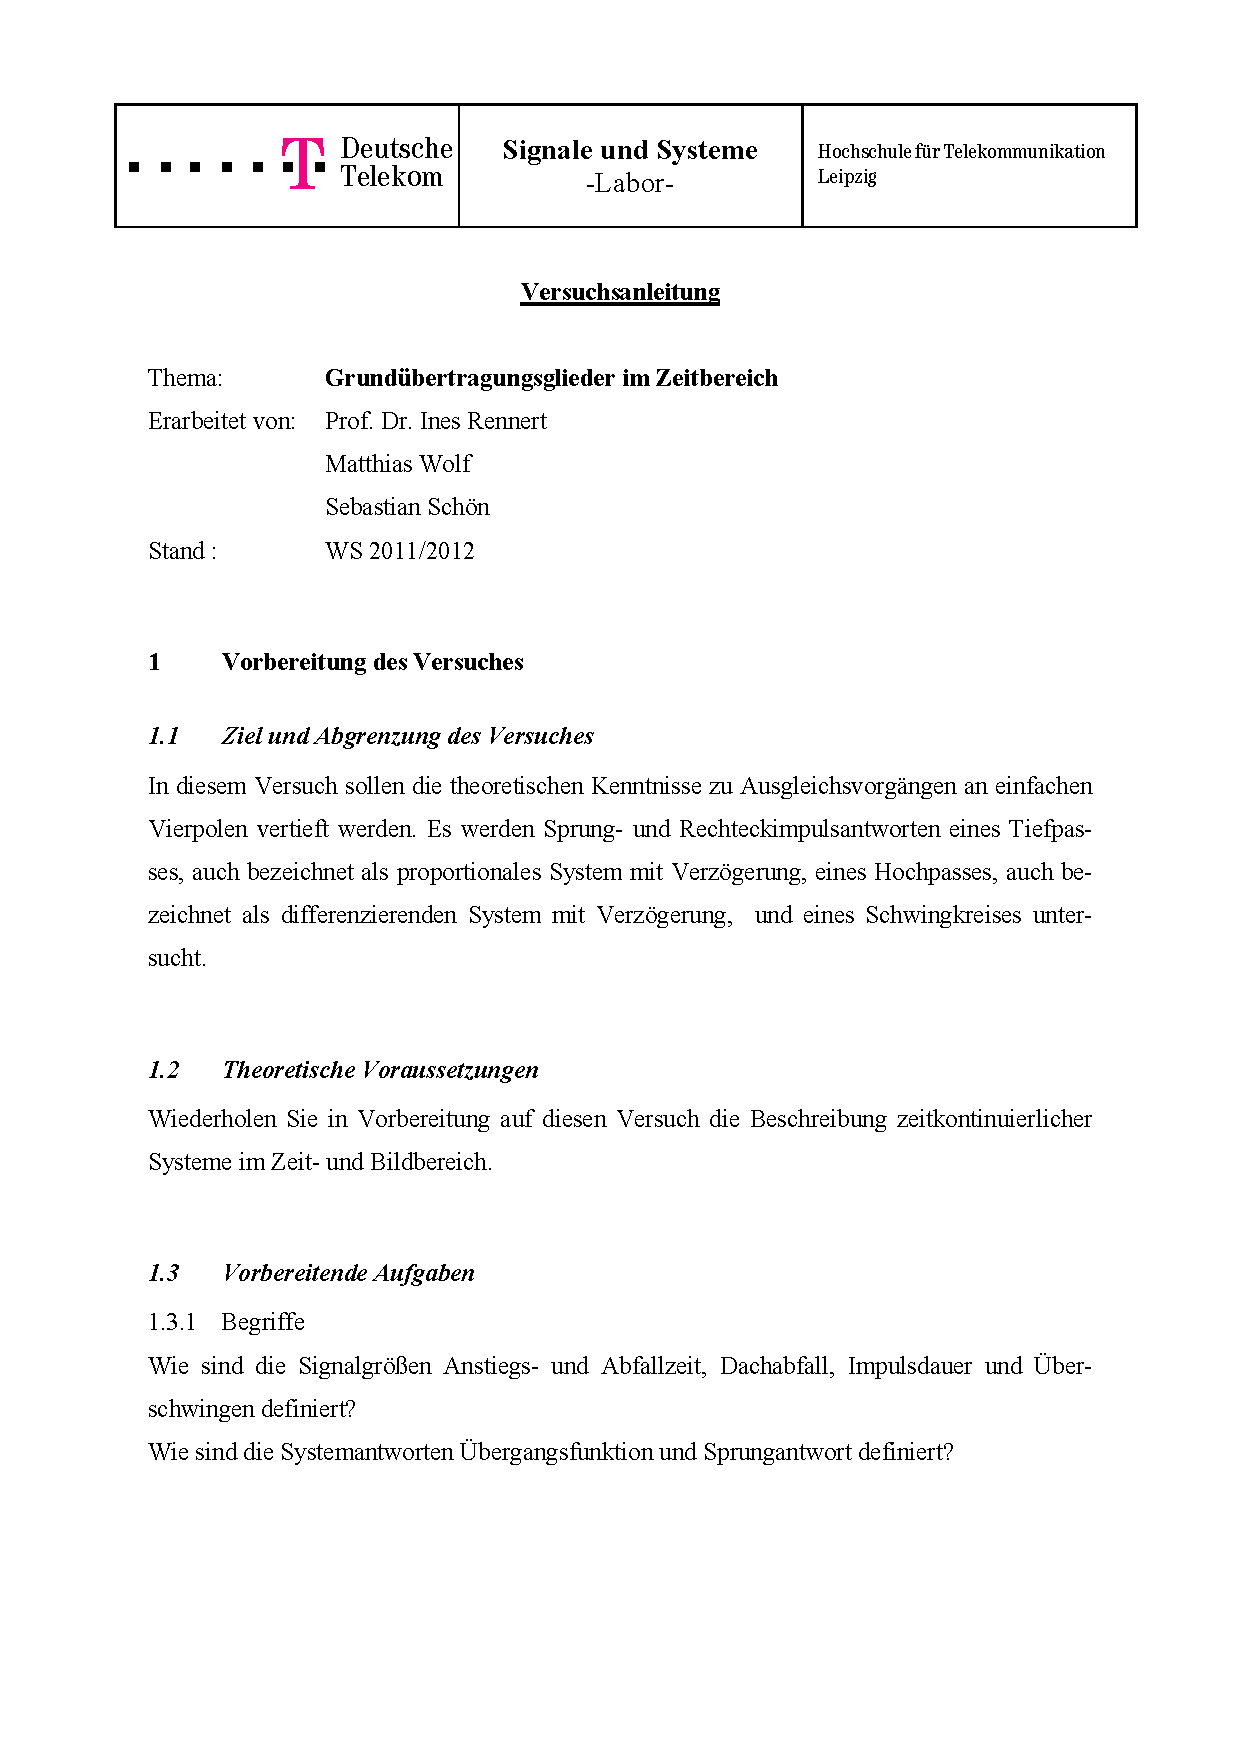
\includegraphics[width=1.0\textwidth]{Bilder/Grundubertragungsglieder im Zeitbereich (verschoben)}\newpage
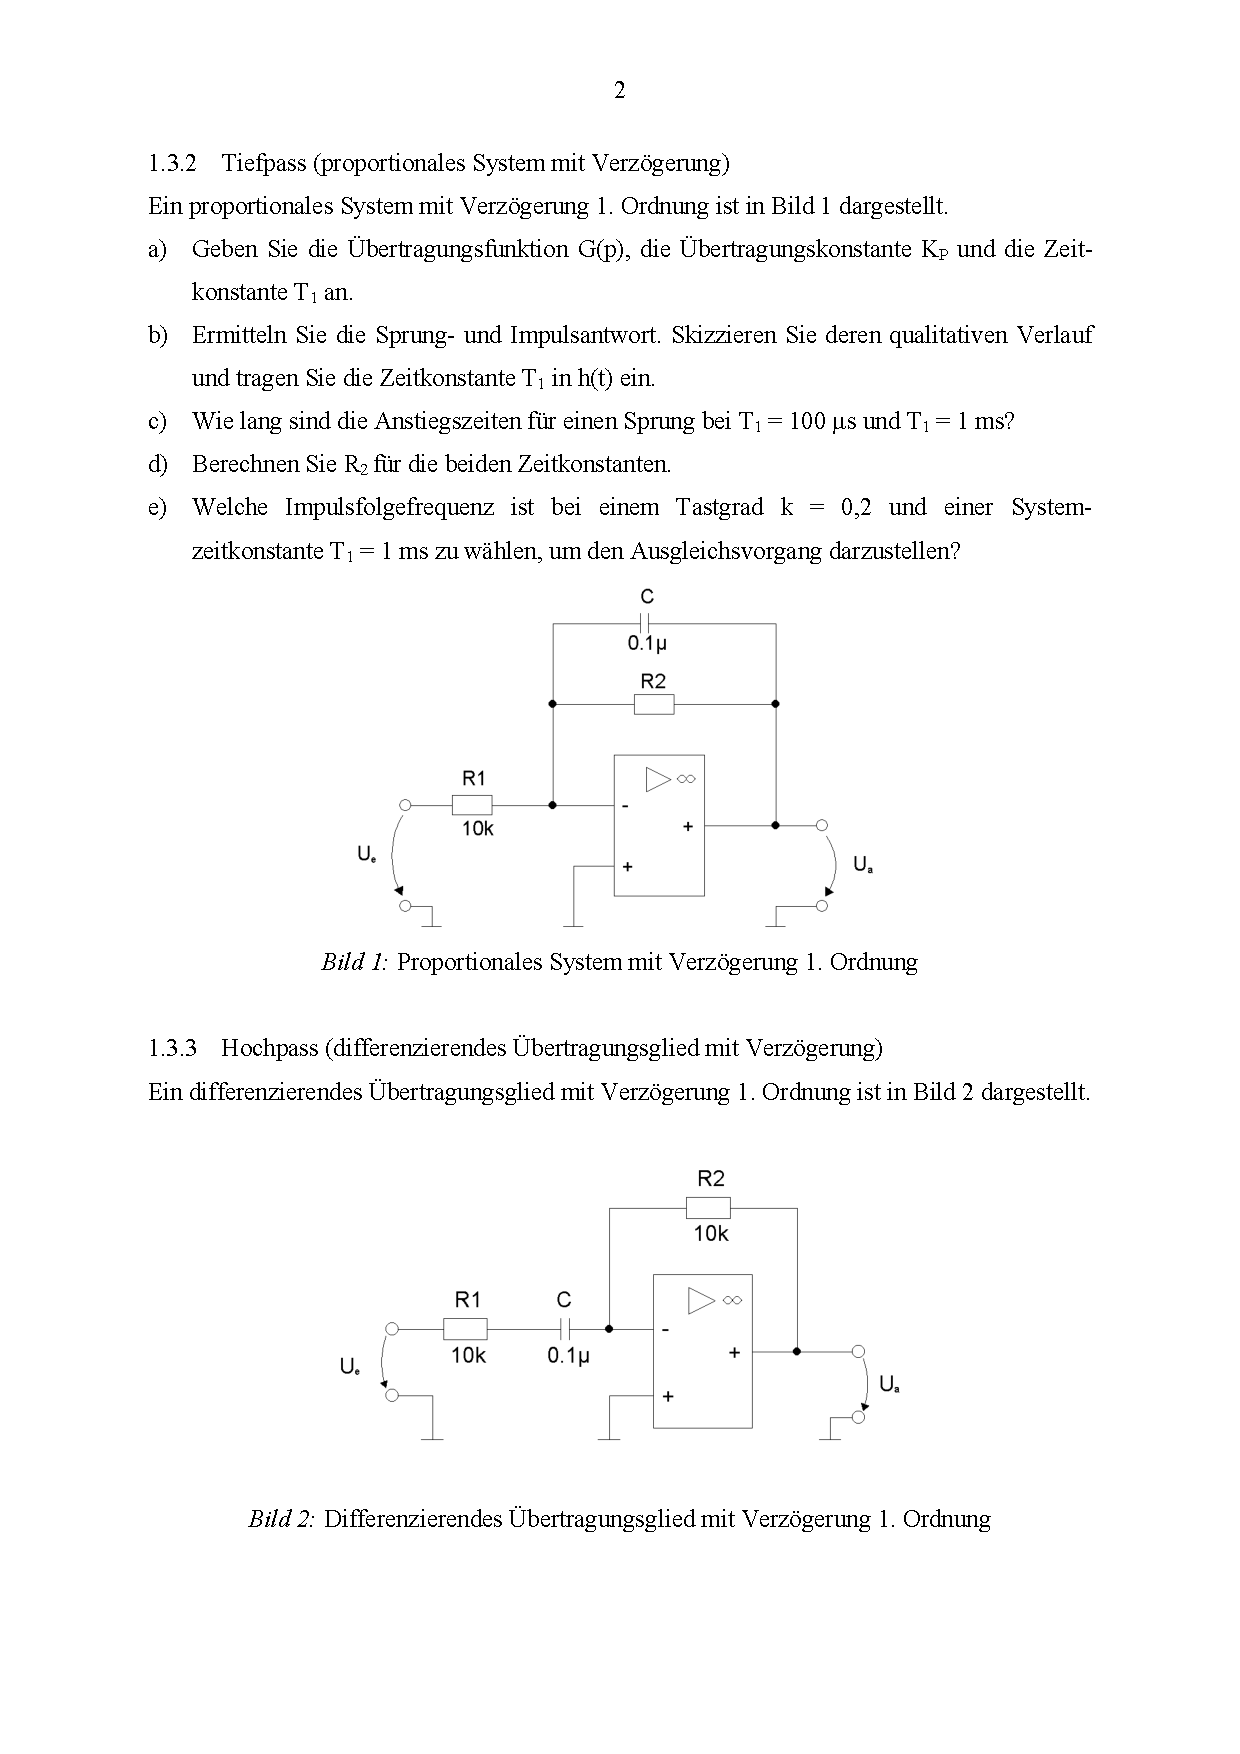
\includegraphics[width=1.0\textwidth]{Bilder/Grundubertragungsglieder im Zeitbereich (verschoben) 2}\newpage
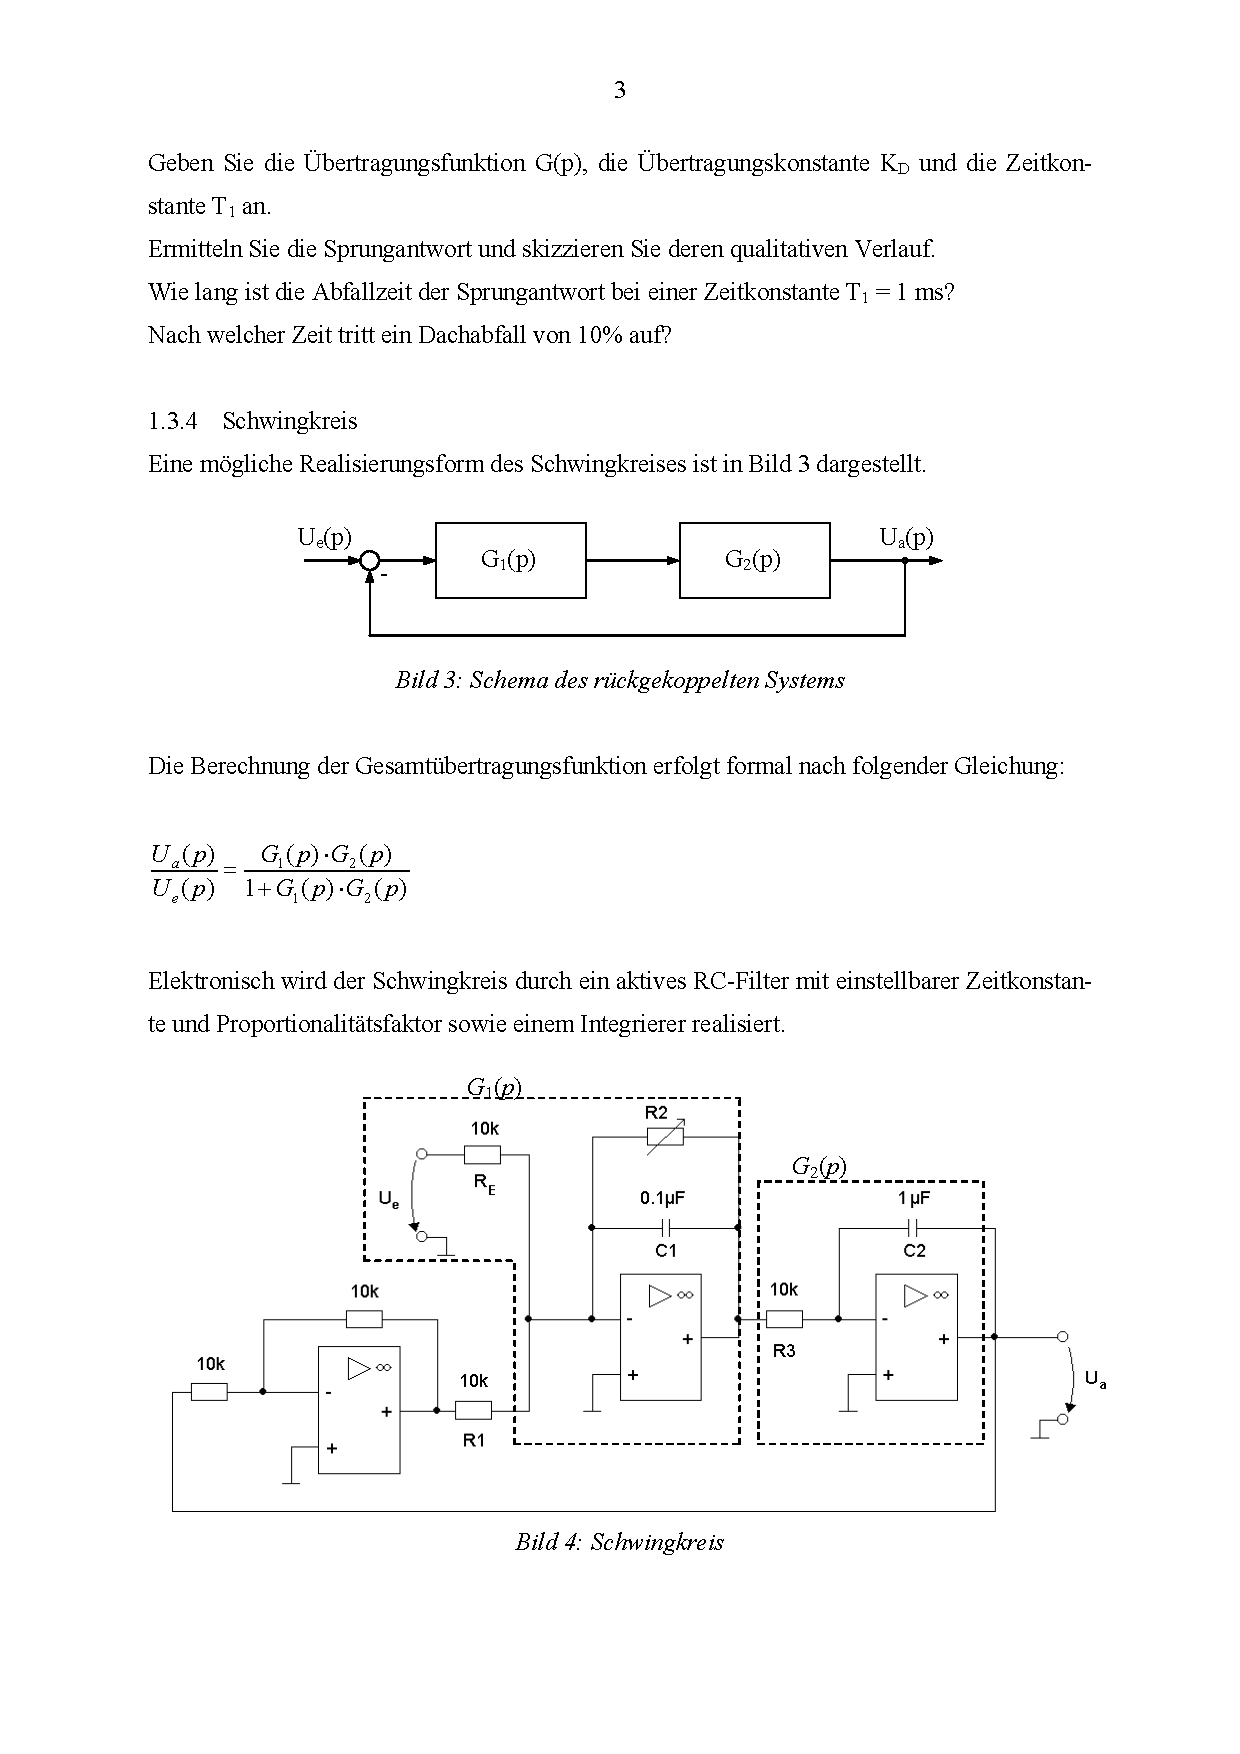
\includegraphics[width=1.0\textwidth]{Bilder/Grundubertragungsglieder im Zeitbereich (verschoben) 3}\newpage
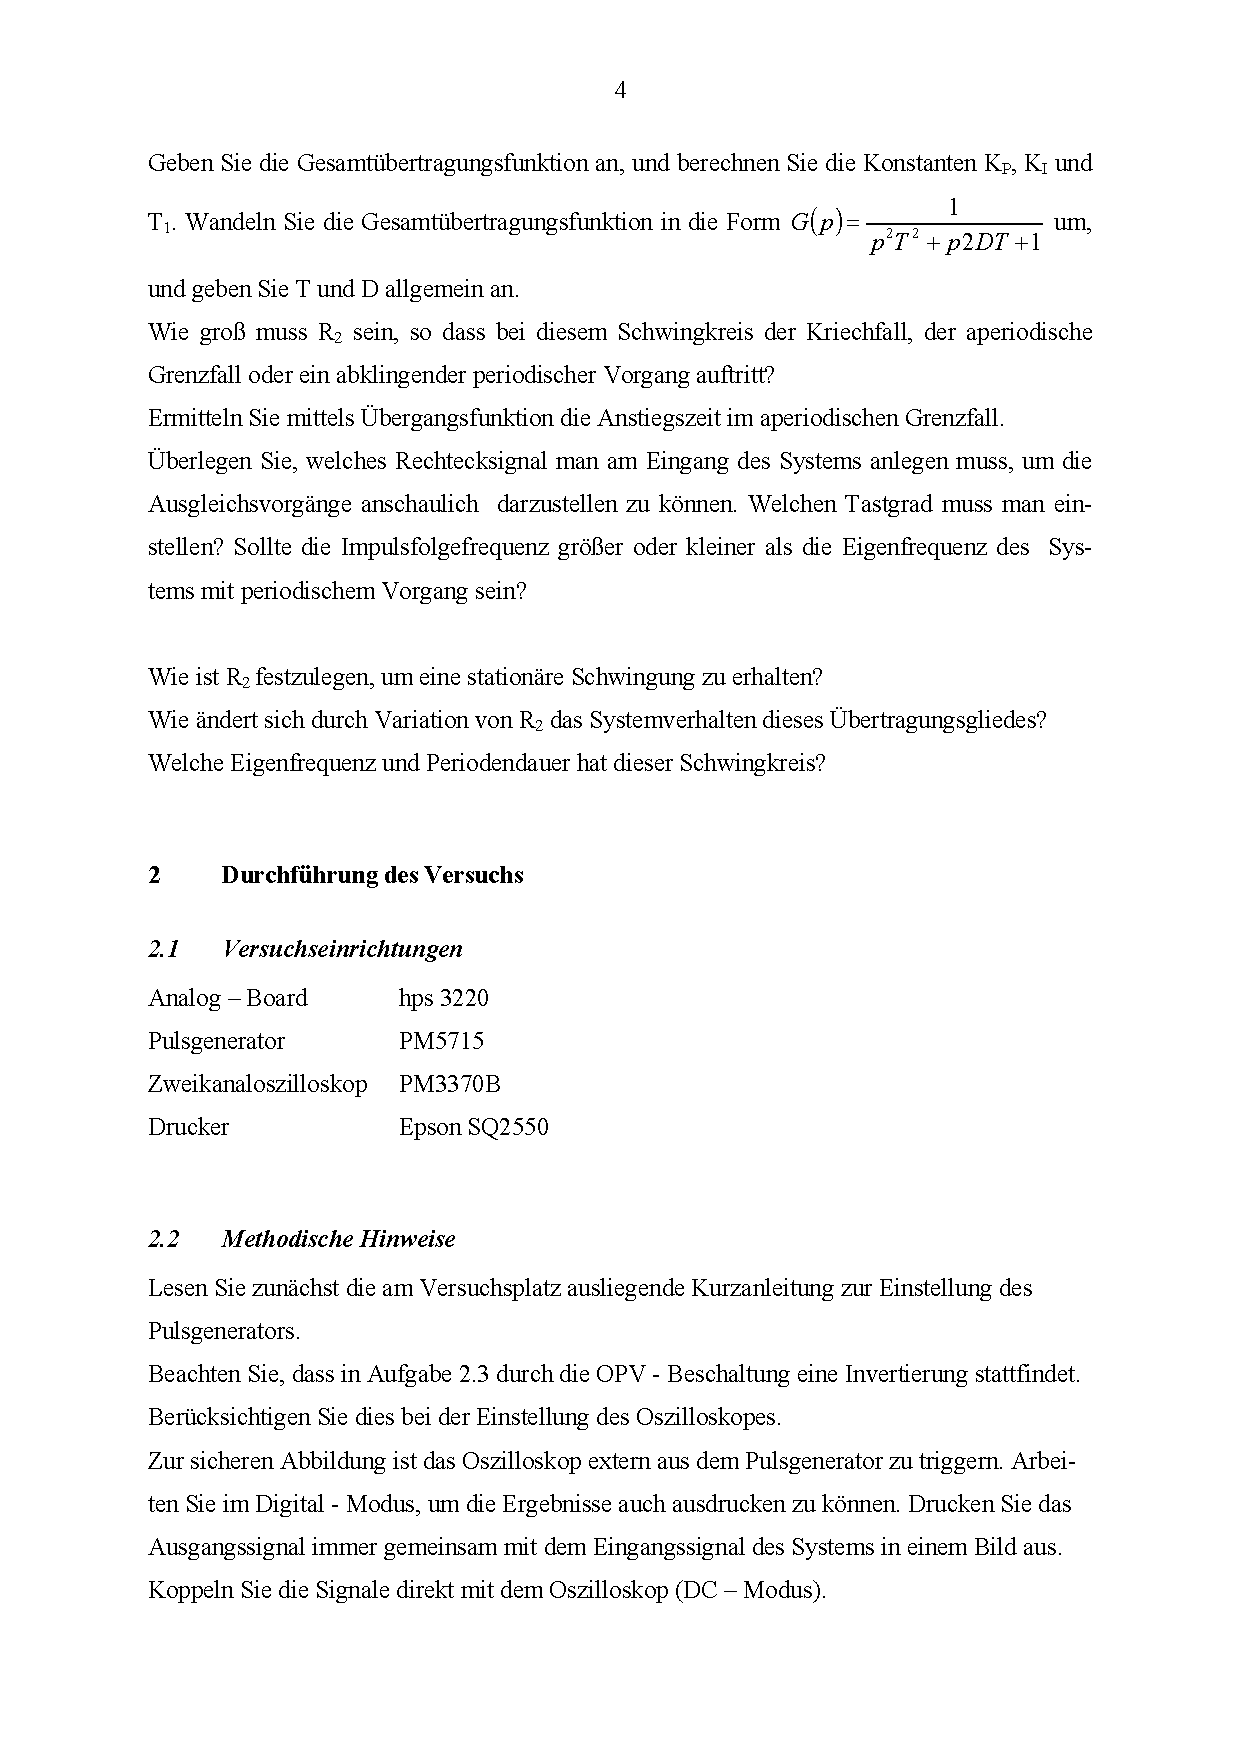
\includegraphics[width=1.0\textwidth]{Bilder/Grundubertragungsglieder im Zeitbereich (verschoben) 4}\newpage
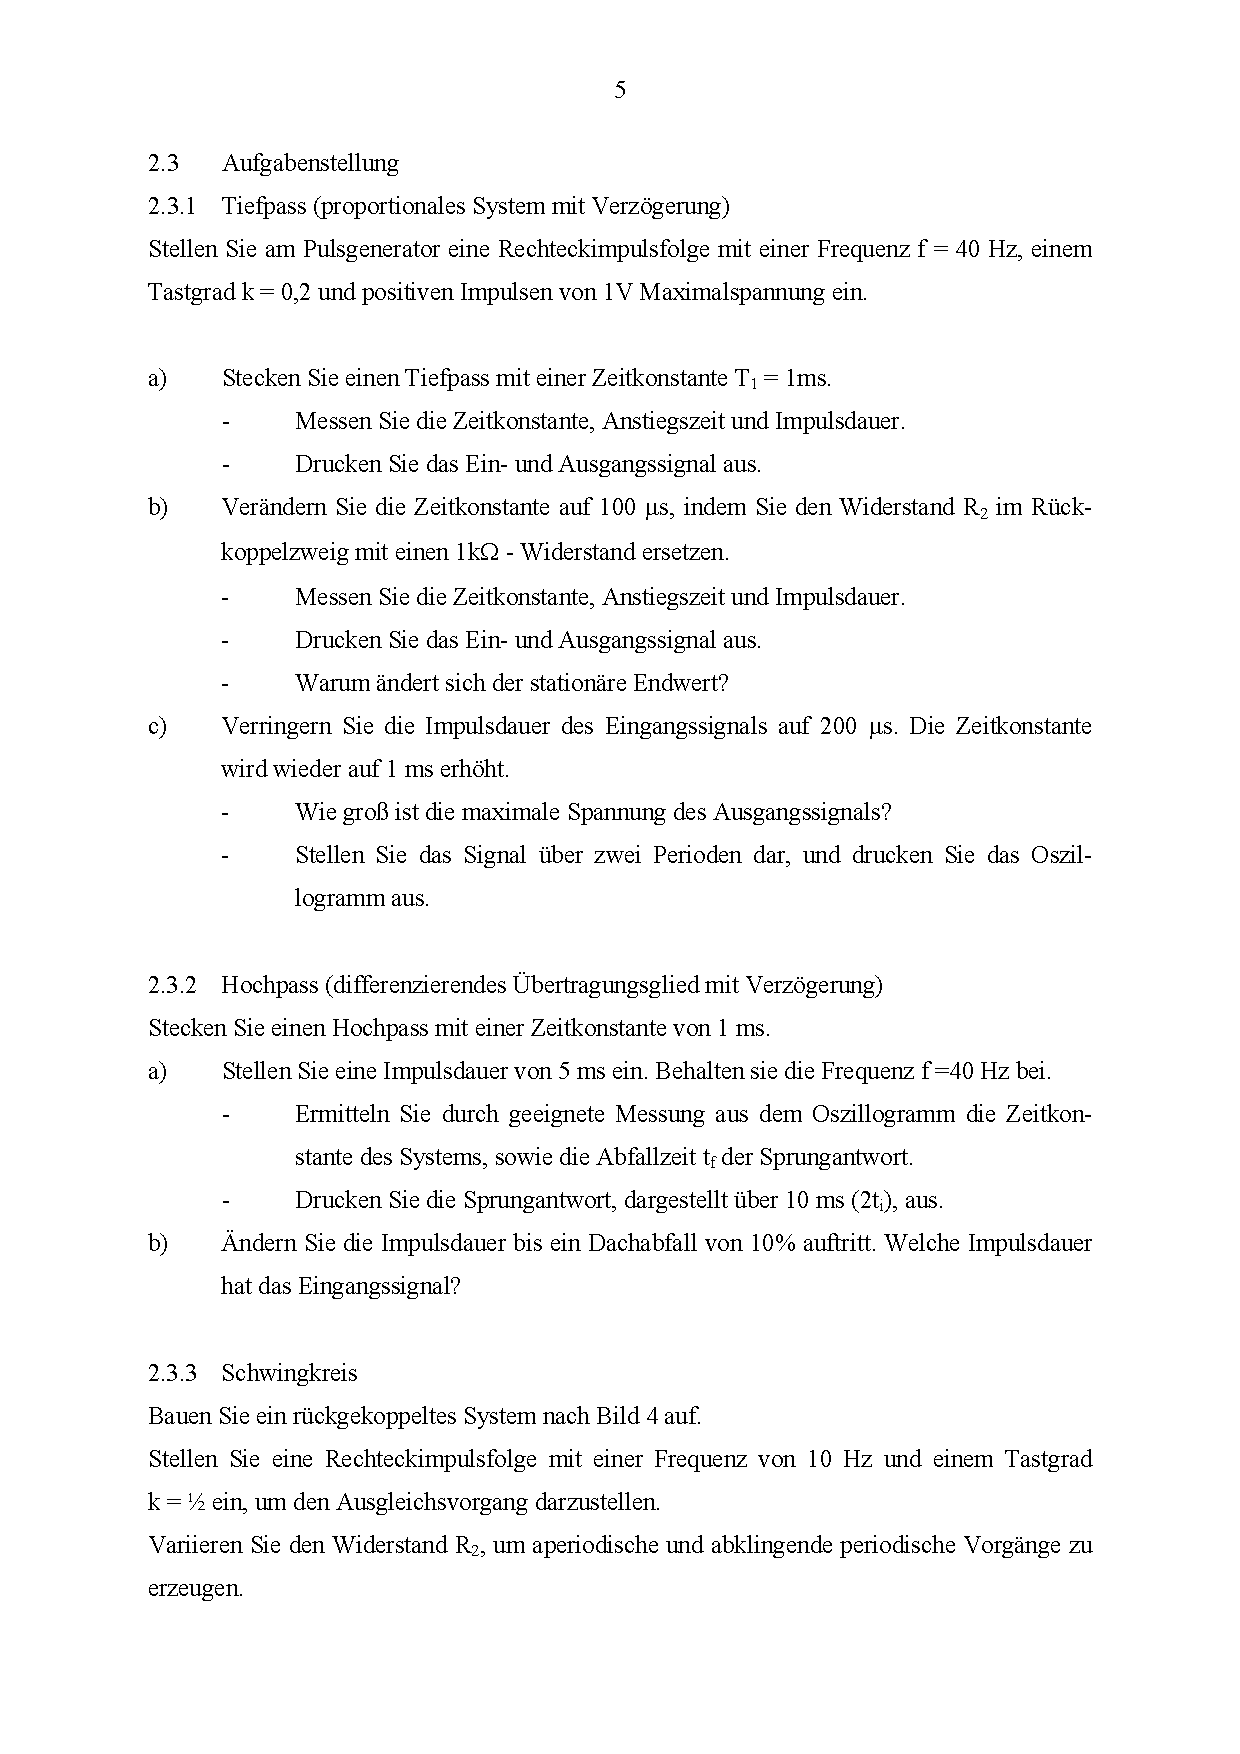
\includegraphics[width=1.0\textwidth]{Bilder/Grundubertragungsglieder im Zeitbereich (verschoben) 5}\newpage
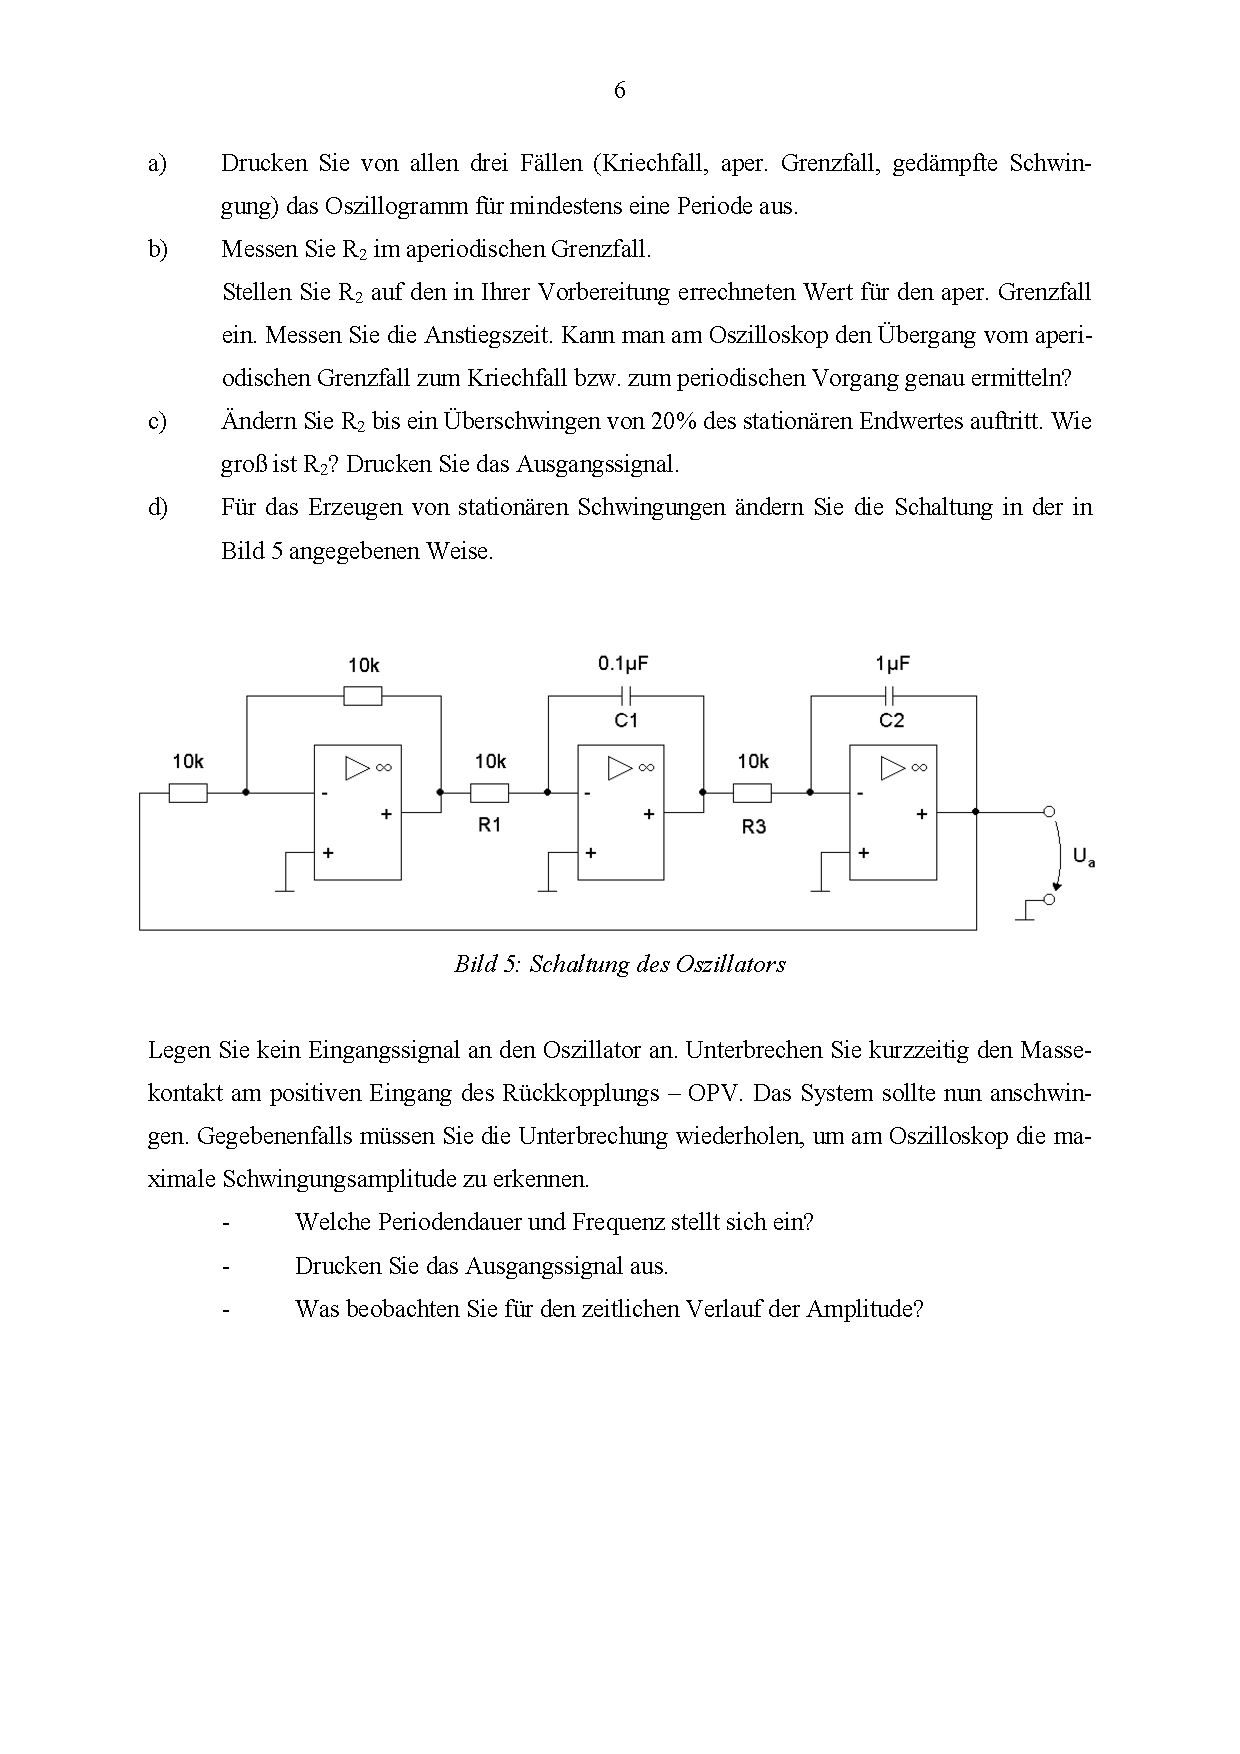
\includegraphics[width=1.0\textwidth]{Bilder/Grundubertragungsglieder im Zeitbereich (verschoben) 6}\newpage
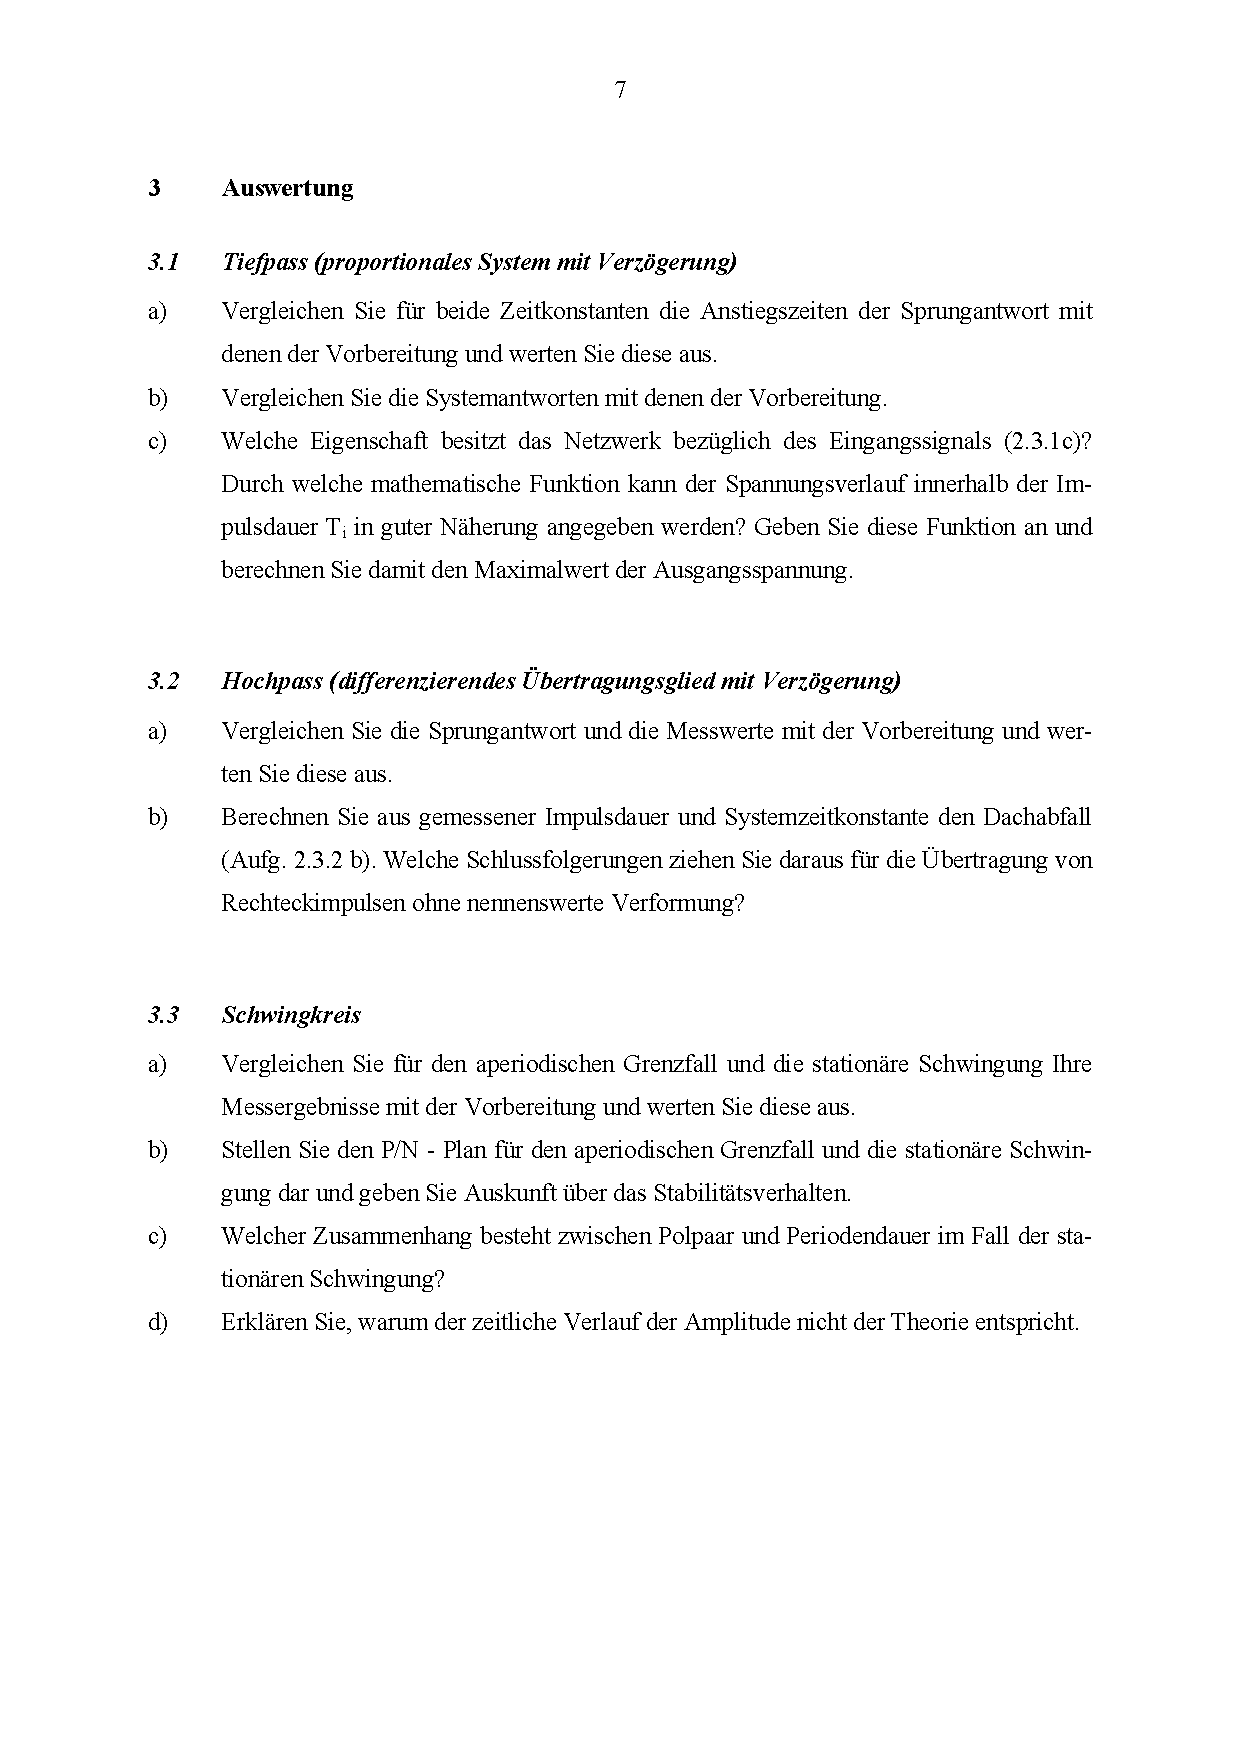
\includegraphics[width=1.0\textwidth]{Bilder/Grundubertragungsglieder im Zeitbereich (verschoben) 7}\newpage


\section{Vorbereitung des Versuches}
\subsection{Ziel und Abgrenzung des Versuches}
\subsection{TheoretischeVoraussetzungen}
\subsection{Vorbereitende Aufgaben}
\subsubsection{Begriffe}
\subsubsection{Tiefpass (proportinales System mit Verzögerung)}
\subsubsection{Hochpass (differenzierendes Übertragungsglied mit Verzögerung)}
\subsubsection{Schwingkreis}
\section{Durchführung des Versuchs}
\subsection{Versuchseinrichtung}
\subsection{Methodische Hinweise}
\subsection{Aufgabenstellung}
\subsubsection{Tiefpass (proportinales System mit Verzögerung)}
\subsubsection{Hochpass (differenzierendes Übertragungsglied mit Verzögerung)}
\subsubsection{Schwingkreis}
\section{Auswertung}
\subsection{Tiefpass (proportinales System mit Verzögerung)}
\subsection{Hochpass (differenzierendes Übertragungsglied mit Verzögerung)}
\subsection{Schwingkreis}

